\slajdid{09_3-s046}
\begin{frame}[label=09_3-s046]{CMOS izlaz sa tri stanja}
% element: 09_3-s046:e01
% element: 09_3-s046:e02
% element: 09_3-s046:e03
% element: 09_3-s046:e04
\begin{columns}[c,onlytextwidth]\column{.47\textwidth}
\begin{center}
{\RazaviSetup
\ctikzset{transistors/scale=.60}\begin{tikzpicture}[line width=.7pt,x=.55cm,y=.48cm,font=\sitneoznake,>=Latex]\begin{scope}[shift={(0,5.4)}]\node[rz pmos,nobulk,anchor=S] (M1) at (.4,.65) {};\draw[wire](M1.D)--(.4,-.65);\draw[wire](-1,0)node[left]{} -| (M1.G);\end{scope}\node[right]at(.5,5.4){P};\begin{scope}[shift={(0,0.6)}]\node[rz nmos,nobulk,anchor=D] (M2) at (.4,.65) {};\draw[wire](M2.S)--(.4,-.65);\draw[wire](-1,0)node[left]{} -| (M2.G);\end{scope}\node[right]at(.5,.6){N};\begin{scope}[DEcrvena]\begin{scope}[shift={(0,3.9)}]\node[rz nmos,nobulk,anchor=D] (M3) at (.4,.65) {};\draw[wire](M3.S)--(.4,-.65);\draw[wire](-1,0)node[left]{} -| (M3.G);\end{scope}\begin{scope}[shift={(0,2.1)}]\node[rz nmos,nobulk,anchor=D] (M4) at (.4,.65) {};\draw[wire](M4.S)--(.4,-.65);\draw[wire](-1,0)node[left]{} -| (M4.G);\end{scope}\draw(-1,3.9)--(-1,2.1);\draw(-1.45,3)node[ocirc]{}node[left]{E}--(-1,3);\end{scope}
\draw(.4,6.05)--(.4,6.35);\draw(.05,6.35)--(.75,6.35)node[above left]{$V_{DD}$};\draw(.4,4.75)--(.4,4.55);\draw(.4,3.25)--(.4,2.75);\draw(.4,1.45)--(.4,1.25);\draw(.4,-.05)--(.4,-.45)node[ground]{};
\draw(-1,5.4)--(-2,5.4)--(-2,.6)--(-1,.6);\draw(-2.5,3)node[ocirc]{}node[left]{A}--(-2,3);\draw[DEcrvena](.4,3)--(1.1,3)node[ocirc]{}node[right]{Y};
\end{tikzpicture}

}

\end{center}
\column{.49\textwidth}
\begin{center}
\begin{tabular}{c|c|c}A&E&Y\\\hline A&0&Z\\A&1&$\overline A$\end{tabular}
\end{center}\begin{center}
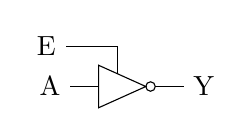
\begin{tikzpicture}[x=.6cm,y=.6cm,font=\sitneoznake]
\draw(0,-.45)--(1,0)--(0,.45)--cycle;\draw(1.1,0)circle(.1);\draw(-.6,0)node[left]{A}--(0,0);\draw(1.2,0)--(1.8,0)node[right]{Y};\draw(.4,.27)--(.4,.85)--(-.7,.85)node[left]{E};\end{tikzpicture}

\end{center}\alert{$Z$ nije vrednost Bulove algebre.}\par
Dva dodatna nMOS tranzistora: $E=0$ → zakočeni; $E=1$ → omogućeno provođenje.
\[t_{pLZ},\quad t_{pHZ},\quad t_{pZL},\quad t_{pZH}\]
\end{columns}\Rezultat{Izlaze smemo povezati ako je samo jedno kolo van stanja visoke impedanse.}
\end{frame}
